\chapter{Experimental Evaluation}
\label{chapter:experiments}

In this chapter we present experimental results of the method proposed. We designed three sets of experiments for evaluation. 

In the first set of experiments we compared plain POMDP formulation and POMDP decomposition models. The goal of this experiment set is to understand the overhead of POMDP decomposition method and compare this overhead with the benefit gained.

In the second set of experiments we tested our data analysis method with different permutations of gene expression data and with synthetetic gene expression networks of different connectivity levels from sparse to very dense. The goal of this experiment set is to explored how our method is affected by the nature of the gene regulatory network and gene expression data sampled from this network. 

In the third set of experiments we compared POMDP formulation with similar finite horizon methods. The goal of this experiment set is to verify the benefit of POMDP formulation for the GRN control problem.

\section{Experiments on POMDP Decomposition}\label{exp-res}

In this section, we evaluate the proposed decomposition method by conducting a sequence of experiments to demonstrate its
applicability, effectiveness and efficiency. We start by describing the implementation and the testing
environment. Then we present an illustrative example. Finally we report and analyze the test result.

We used two synthetic networks and one real network in the experiments. For each of the two networks, the
gene expression data is generated using the method proposed by Yu et al.~\cite{Yu02}. For solving the POMDP
problems, we used symbolic Perseus, a factored POMDP solver developed in Matlab by Pascal Poupart
\cite{Poupart05}. The main policy generator uses symbolic Perseus extensively; it has been coded partially in
Matlab and Ruby. All other modules of the system are coded in Ruby (jruby 1.4.0).

The execution times presented in the reported results have two components, problem preparation phase and
execution phase. The problem preparation phase was run on AMD Turion x2 1.8Ghz CPU/1GB RAM and Intel Core 2
Duo E4600 2.4 Ghz CPU/4GB RAM configuration computer; and the problem solution phase was run on Intel Core 2
Duo E4600 2.4 Ghz CPU/4GB RAM configuration computer.

\begin{figure}
\centering
  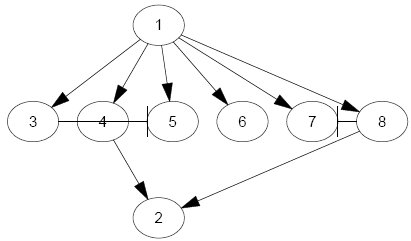
\includegraphics[scale=0.305]{experiments/grn1.jpg}
  \caption{Example gene regulatory network}\label{figure:grn1}
\end{figure}
\subsection{An Example Decomposition and Execution}
\label{section:example} Shown in Figure~\ref{figure:grn1} is one of the synthetic GRNs used in the
experiments. In this subsection, we will use this network to illustrate and demonstrate the decomposition and
execution~phases.We typically defined gene $2$ to be a target gene in our experiments. Note that genes $5,6$ and $7$ in this network do not effect the expression level of gene $2$. So, we predicted our approach could decompose the problem such that these genes could be eliminated.

Assume that in the network shown in Figure~\ref{figure:grn1} the control problem is defined such that
gene~$1$ is the input gene and gene~$2$ is the target gene to be promoted. In Section~\ref{section:dataanalysis},
we presented an example of similarity analysis based on gene expression data. Here we will not go into the
details of the gene expression data analysis, instead we will consider two different scenarios with two
possible partitioning schemes extracted after the data analysis.

For the first scenario, consider a partition of genes, say $P_1$, extracted via gene expression data
analysis, where $P_1 = \{\{1,2,3,4,6,8\},\{5,7\}\}$. Then the problem will be divided into two subproblems,
one subproblem for genes $\{1,2,3,4,6,8\}$ and another subproblem for genes $\{5,7\}$. For the first
subproblem, the goal gene is~$2$ and the input gene is~$1$. These genes are from the input and goal sets of
the main problem. For the second subproblem, there is no goal gene or input gene, since genes $5$ and $7$ are
neither in the goal nor in the input set of the main problem.

Note that gene $5$ is controlled by genes~$1$ and~$3$; and gene~$7$ is controlled by gene~$8$. So, the second
subproblem is controlled by some genes in the first subproblem; however, the inverse is not true. Genes~$5$
and~$7$ do not influence any gene in the first subproblem. For the first step in coordinating the
subproblems, we enumerate the subproblems to be solved. The first subproblem has some goal description
(promoting gene~$2$), so it is marked ``to be solved''. The second subproblem does not have any goal
description; so it is not marked ``to be solved''. Then, we explore whether the first subproblem is
controlled by the second subproblem; because the result of the check is negative, no other subproblem is
marked ``to be solved''. Therefore, the first subproblem is the only subproblem we should solve. In the
execution part, we simply solve the first subproblem and use the policy returned.

As a more complex scenario, consider another partition of genes $P_2$ extracted via gene expression data
analysis, where $P_2 = \{\{1,3,5,6\},\{2,4,7,8\}\}$. Then the problem will be divided into two subproblems,
one subproblem for genes $\{1,3,5,6\}$ and another subproblem for genes $\{2,4,7,8\}$. Note that genes $4,7$
and $8$ are controlled by gene $1$. So the second subproblem is controlled by some genes in the first
subproblem. However, the inverse is not true. Genes $2,4,7$ and $8$ do not influence any gene from the first
subproblem. For the first step in coordinating the two subproblems, we enumerate the subproblems that should
be solved. The first subproblem does not have any goal description, so it is not marked ``to be solved''. The
second subproblem has some goal description (promoting gene $2$) so it is marked ``to be solved''. Then, we
explore whether the second subproblem is controlled by the first subproblem. Since the first subproblem
controls the second subproblem, the first subproblem is also marked ``to be solved''.

Now both subproblems should be solved. The influenced genes $4,7$ and $8$ are added to the first subproblem
as target genes. The first subproblem now contains genes $1,3,4,5,6,7,8$. The three genes $4,7$ and $8$ are
also input genes for the second subproblem. The second subproblem is solved for a policy governing genes
$4,7$ and $8$. Since in this work we do not make use of joint actions, each action in this policy will govern
the expression level of a single gene and there are six possible actions, namely $gene_4 = on$, $gene_4 =
off$, $gene_7 = on$, $gene_7 = off$, $gene_8 = on$ and  $gene_8 = off$. Each of these six case is a goal
description for the first subproblem; however some of the actions might not be used in the policy. Assume
these three actions are used in the policy $gene_4 = on$,  $gene_7 = off$ and $gene_8 = on$; accordingly, we
solve three copies of the first problem, each with a single goal description corresponding to one of these
actions.

Finally, our policy is simply a glued version of policies from the two problems. When we need to execute the
action $gene_4 =on$, instead we execute the action in the policy of the first subproblem (with goal
description $gene_4 = on$), we use observations from the second problem to decide on an action in the policy
of the second problem and observations from the first problem to decide on an action in the policy of the
first problem.

\subsection{General Outline of the Quantitative Experiments}
In the following subsection, we present and discuss the results of the conducted experiments. We have conducted two sets
of experiments for analyzing the performance of our method. The first group of experiments are performed
using two random synthetic GRNs and the gene expression data sampled from these networks. We defined a control
problem on each network, and we used gene expression data samples of different sizes to solve the control
problems by using our method. For each result set, the outcome from the two control problems defined on the
two GRNs are presented together.

The second group of experiments are based on gene profiling data produced from a study of metastatic melanoma
by Bittner et al.~\cite{Bittner00}. This data contains 31 samples of 587~genes. Kim et al.~\cite{Kim02} first
studied this data for finding a PBN representation of the GRN. It is computationally intractable to use all
the genes for the control problem. So, they detected the 10~most relevant genes and built a PBN of these 10
genes. Datta et al.~\cite{Datta03} and Bryce et al.~\cite{Bryce07} separately used this same data in their
studies; they separately formulated partially observable control problems. Datta et al. used a seven genes
GRN. We used both the ten genes and the seven gene networks in our experiments. These networks are actually
wiring diagrams of the PBNs, where each gene is influenced by 3-4 other genes. We also used sparser versions
of these networks, where all bidirectional connections are dropped. We present the results from the second
group of experiments in the next subsection where we discuss the performance of our method relative to the
works of Datta et al.~\cite{Datta03} and Bryce et al.~\cite{Bryce07}.

For all the experimental cases, we present two sets of results from two problems. The first problem uses only
the POMDP formulation method and a policy is generated by solving a single POMDP. The second problem applies
the whole POMDP decomposition method outlines in the paper. In the first problem, the policy generated by our
method is identical to the policy generated from the original POMDP problem. Thus, the results related to
this problem can be interpreted as worst case scenario. In the second problem, we observed smaller policies
generated in less time. Thus, this problem can be interpreted as a best case scenario, where maximum benefit
from our approach is reported.

There are also two sets of separate experiments used to explore the impact of network connectivity and data order to our approach. For experiments on data order, we used the metastatic melanoma data and generated permutations of this data as explained in the corresponding subsection. For experiments related to network connectivity we generated randomly connected and directed graphs and constructed gene regulatory networks by slightly modifying these graphs.

\begin{figure}[h!]
\centering
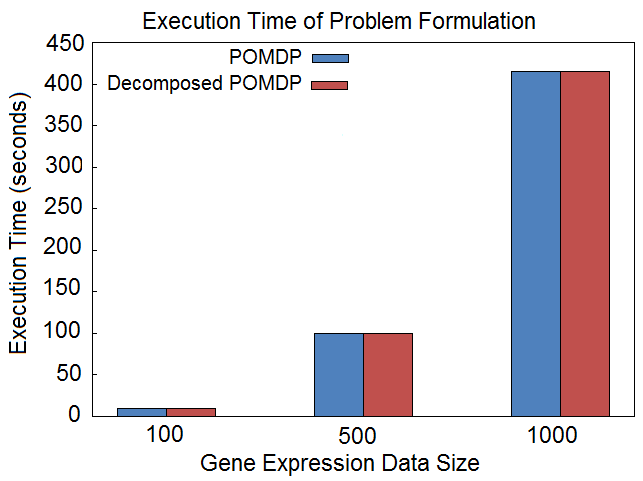
\includegraphics[scale=0.5]{experiments/graph1.png}
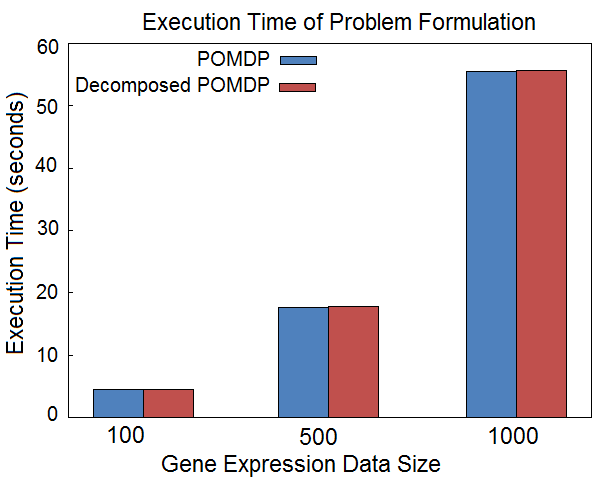
\includegraphics[scale=0.5]{experiments/graph2.png} %}
\caption{Problem formulation module
execution times for two different networks}\label{figure:formulationgraph}
\end{figure}

\begin{figure}[h!]
\centering
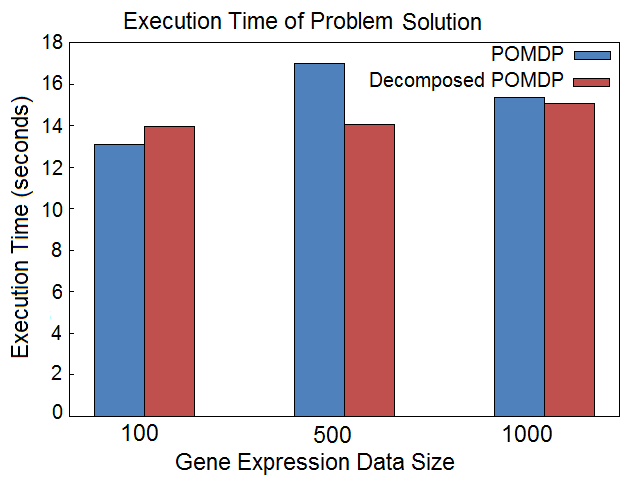
\includegraphics[scale=0.5]{experiments/graph3.png}
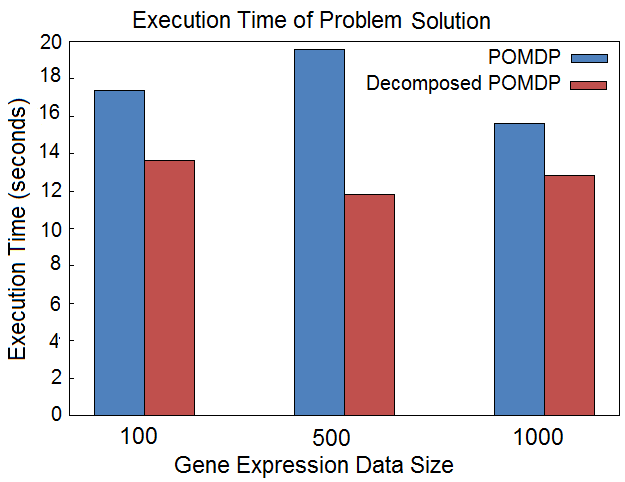
\includegraphics[scale=0.5]{experiments/graph4.png}
\caption{Execution times for policy generation}\label{figure:policygeneration}
\end{figure}

\subsection{Experiments on Synthetic GRNs}
The problem formulation costs are shown in Figure~\ref{figure:formulationgraph}. POMDP result set is the
computational cost of constructing the main POMDP problem in seconds. Decomposed POMDP result set is the
computational cost of formulating the control problem in decomposed POMDP format. Note that the latter
process requires first formulating the main problem, thus the actual cost of decomposing the main problem is
the difference between the two bars, which is quite small. The dominating factor in both formulations is the
gene expression data analysis. For a data set of 1000 samples, due to the cost of this analysis, the
execution time goes up to 6 minutes. However, on average it is possible to conclude that the analysis and the
problem formulation are completed in a reasonable amount of time. These result sets clearly show that the
overhead of decomposing the POMDP problem is very small.

Figure~\ref{figure:policygeneration} shows the execution times used for constructing the policies. This
result set may be considered as the most important result because the main goal of our approach is to solve
the GRN control problem more efficiently. Note that for the first problem, the execution times are close; our
approach is performing slightly better for larger gene expression data sets. However, for the second problem,
the execution cost of our approach is clearly much less than the plain POMDP method. The structure of the
decomposed problem in the second network is very similar to the first example presented in
Section~\ref{section:example}. The problem is decomposed into two pieces; we could completely omit one of the
pieces, and this leads to a smaller single POMDP problem. However, the first problem is decomposed into four
pieces, which are closely related to each other (thus forming loops in the subproblem dependency graph). Thus
all the subproblems are re-combined again and the performance is very similar to the original problem. This
result set clearly shows that applying our method could possibly lead to significant gain in performance for
problems with loosely coupled state variables.

For both control problems, 500~runs have been carried out, mainly for determining the quality of
the policies generated. The length of the simulations are also recorded in order to understand any
performance gain or loss introduced by our approach.

\begin{figure}[h!]
\centering
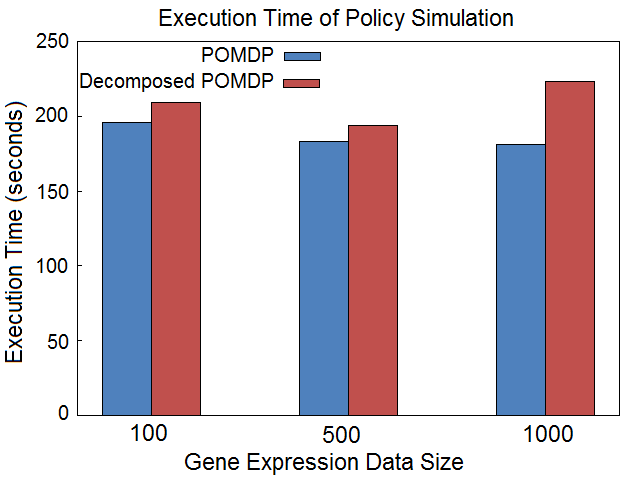
\includegraphics[scale=0.5]{experiments/graph5.png}
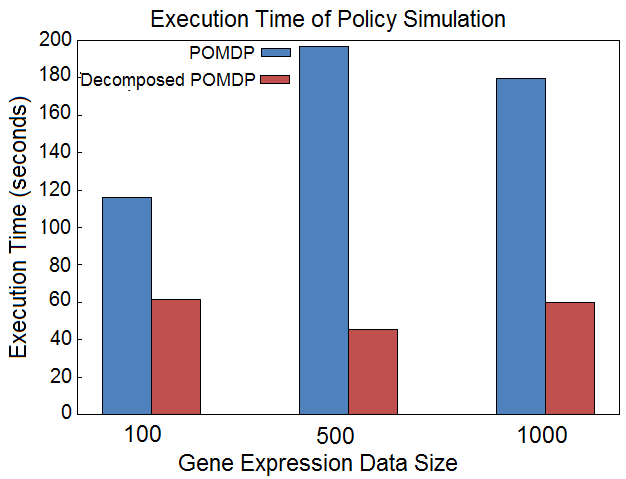
\includegraphics[scale=0.5]{experiments/graph6.png}
\caption{Execution times for policy execution}\label{figure:policyexecution}
\end{figure}
\begin{figure}[h!]
\centering
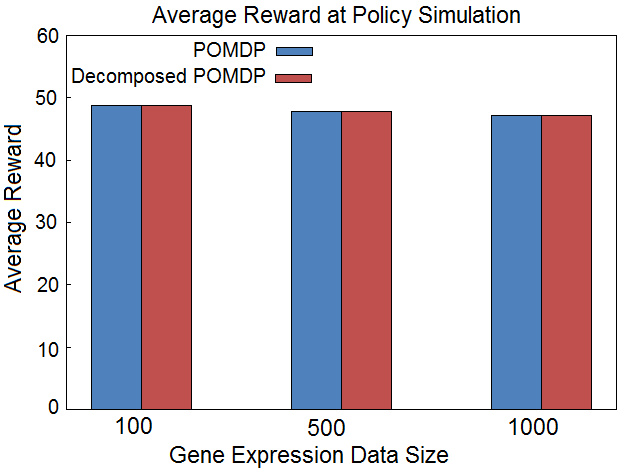
\includegraphics[scale=0.5]{experiments/graph7.png}
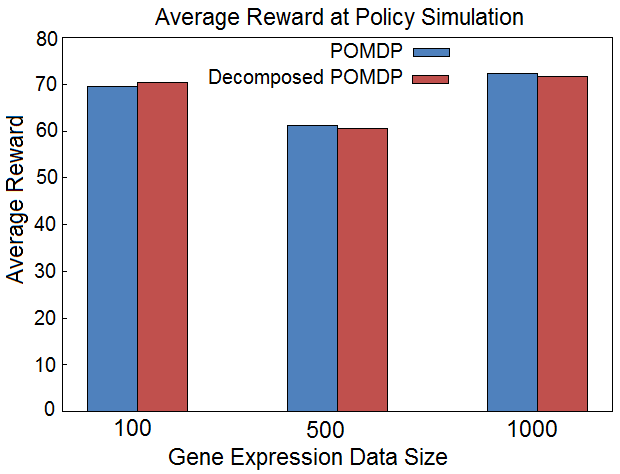
\includegraphics[scale=0.5]{experiments/graph8.png}
\caption{Average Rewards}\label{figure:averagereward}
\end{figure}
Figure~\ref{figure:policyexecution} presents the lengths of the simulations. For the first network, the
lengths of the simulations are close; our approach is performing slightly worse. This slight decrease in
performance is expected since similar policies are generated for this problem. The difference in the
performance can be explained by the overhead of our method, which is not so significant compared to the
simulation length. However for the second network, the simulation time drastically decreased to 80\%. The
most important reason behind this increase in performance is the fact that our approach generates a smaller
policy for the problem.

Figure~\ref{figure:averagereward} presents the average reward gained in these simulations. The amount of
reward gained by our method is nearly identical to the amount of reward gained by the single POMDP problem.
By examining these results, we can conclude that our method is producing possibly smaller policies without
any loss in the policy quality. This characteristic of our approach leads to simpler and effective policies.

%%%%%% edited at 4/4/10 %%%%%%%%%%%
By combining all the results, we can conclude that our approach is successful in achieving the performance
goals we established beforehand for the synthetic data we used. Our method produces structured problem
formulations with little overhead. These formulations can be solved in less time with standard POMDP solvers.
The optimality of the resulting policies could be classified as close to that of the generated plain POMDP
policies; however our approach has the capability of producing more compact policies that can be executed
more efficiently.
%%%%%%%% end of edit at 4/4/10 %%%%%%%%%%%

\begin{figure}
\centering 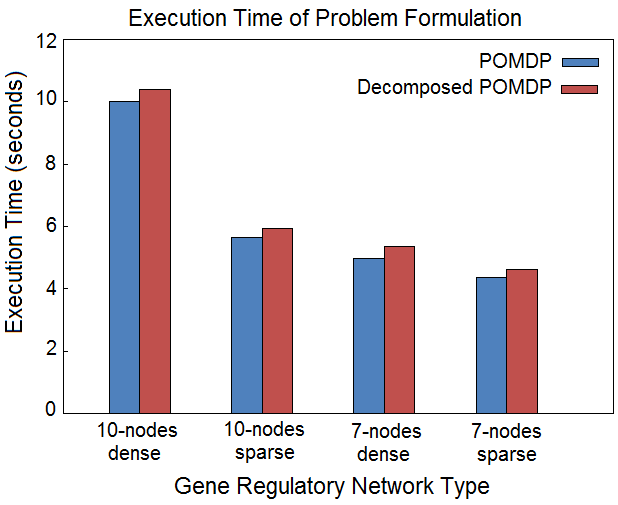
\includegraphics[scale=0.5]{experiments/graph9.png}
\caption{Problem formulation module execution times for four different
networks.}\label{figure:formulationgraph2}
\centering 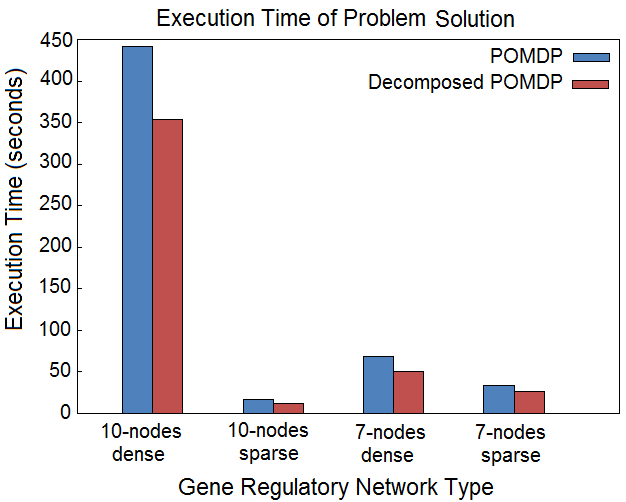
\includegraphics[scale=0.5]{experiments/graph10.png}
\caption{Execution times for policy generation}\label{figure:policygeneration2}
\end{figure}
\begin{figure}
\centering 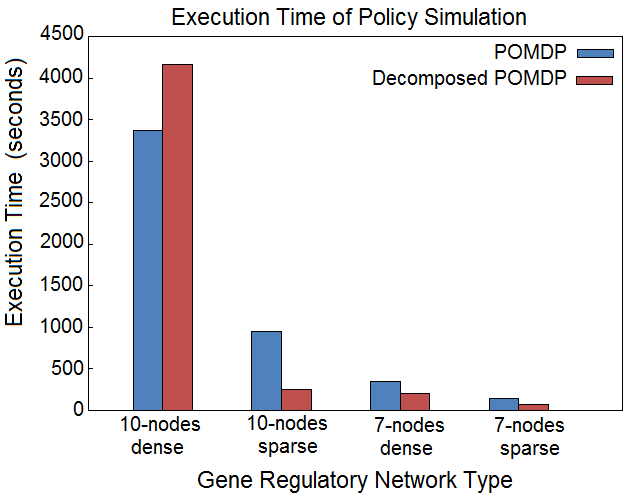
\includegraphics[scale=0.5]{experiments/graph11.png}
\caption{Execution times for policy execution}\label{figure:policyexecution2}
\centering 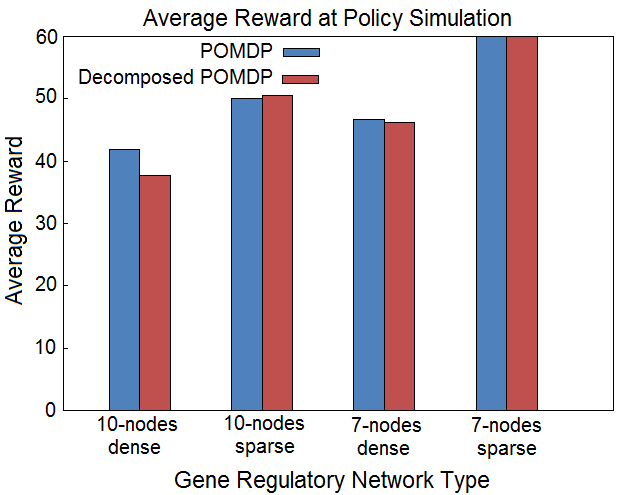
\includegraphics[scale=0.5]{experiments/graph12.png}
\caption{Average Rewards}\label{figure:averagereward2}
\end{figure}
\subsection{Experiments on Real Biological Gene Expression Data}
%%%%%%%%%%%%%% moved from next subsection %%%%%%%%%%%
Figures~\ref{figure:formulationgraph2}~-~\ref{figure:averagereward2} present the execution times for
different stages of the control problem and the average reward collected. The execution times for problem
formulation module are similar to the results of the previous subsection. There is a problem formulation time
around 5 seconds before attempting to solve the problem and the overhead of decomposing the POMDP problem is
small compared to the formulation overhead.

The execution times for policy generation clearly show the benefits of POMDP decomposition as in the previous
subsection. For all networks based on the gene profile data, decomposing the POMDP problem helped in solving
the problem faster. For the sparse networks, using its full potential, our method generates a policy in
around 10 to 20 seconds, even for a 10-genes GRN. Also the average rewards clearly shows that the generated
policies are still close to optimal, even closer than the plain POMDP approach, for all cases. Finally, our
method also succeeded in reducing the time necessary for executing the generated policy. Especially for the
sparse network of 10~genes, our approach successfully reduces the simulation time by nearly 70\%.

\section{Experiments on the Influence of  Gene Expression Data and Gene Regulatory Network}
\subsection{Experiments on Data Order}
Independent from other experimental studies, we also conducted a test for understanding the impact of the order of data. As Section \ref{section:dataanalysis} discusses, the order of samples in our data set has an impact on our window based gene expression data analysis algorithm. 

A trivial way to reduce the impact of ordering, one can theoretically carry on the analysis for all permutations of the data and combine the results as we combined the local results to obtain global similarity values. However this approach is computationally intractible. It is even impossible to test the impact of all different permutations by designing a one shot test. 

Thus we designed a simpler test that considers an arbitrary number of permutations of or data. We used the biological gene expression data we used in previous experiments. We reordered or data samples 10000 times randomly and carried on our gene expression analysis for each of the 10000 permutations. We obtained partitioning of genes for each case.

For our original analysis, which is based on the original ordering of the data, we calculated the average Hamming Distance between our analysis result and the analysis results from 10000 permutations. 

Then we chose 50 permutations among 10000. Each of the 50 permutations are used as an alternative ordering of samples on which gene expression analysis can be applied. For each of the 50 samples we calculated the average Hamming Distance between the analysis result of the permutation and all 10000 analysis results. The results of all 51 cases are shown in Figure \ref{figure:permutations}

\begin{figure}
 \centering 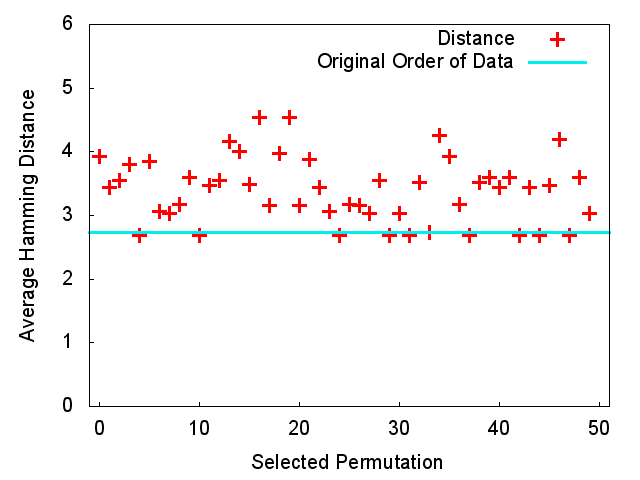
\includegraphics[scale=0.375]{experiments/graph-permutation.png}
\caption{Comparison of solution similarity for different permutations of data samples}\label{figure:permutations}
\end{figure}

Since our data set contains 7 genes and we relabel all the analysis results, maxiumum Hamming Distanve between two analysis results are 6 (first gene is always partitioned to first group). 

The results show that for most of the possible ordering of data, An average Hamming Distance between 3 and 4 exists between the analysis result and all possible analysis results. Only a minority of permutations lead to Hamming Distances greater then 4 or less then 3. 

This shows that a different permutation of data samples might produce different analysis results. However different permutations only show slight deviation from an average case where half of the other possible analysis results are equivalent or very close to the selected permutation and the remaining other half gives different analysis results. 

Moreover our original analysis based on the original ordering of data has an average Hamming Distance of less then 3 to all 10000 permutations (shown with the horizontal line in the Figure). Thus we experimentally verified that analysis result we obtained using the original ordering of the data has the similar statistical properties to a different analysis result produced with a different ordering of data. We can conclude that using the original ordering of the data does not deviate the analysis results much, in fact the analysis results in this case are closer to the other possible results above average.
\subsection{Experiments on Network Connectivity}
Another experiment set we conducted attempts to measure the effect of network connectivity to our method. 

The main focus of our method is to analyze the gene expression data, explore and group genes according to their impack on the control problem to be solved. Genes that have little influnce on the control problem are eliminated totally. According to this perspective it is expectable for our approach to identify such genes more frequently in a sparse network then a dense one. In a dense network each gene is connected to more genes and thus eliminating each gene has a bigger impact on the whole network.

To identify how our approach behaves with different levels of connectivity we generated a seperate set of random gene regulatory networks. These networks are created by modifying randomly generated graphs. They are processed identically with the synthetic gene regulatory networks we used in the experiments. First synthetic gene expression data is created by using these networks, this data is analyzed and the analysis results are used for creating decomposed version of the POMDP problems at hand. 

\begin{figure}
 \centering 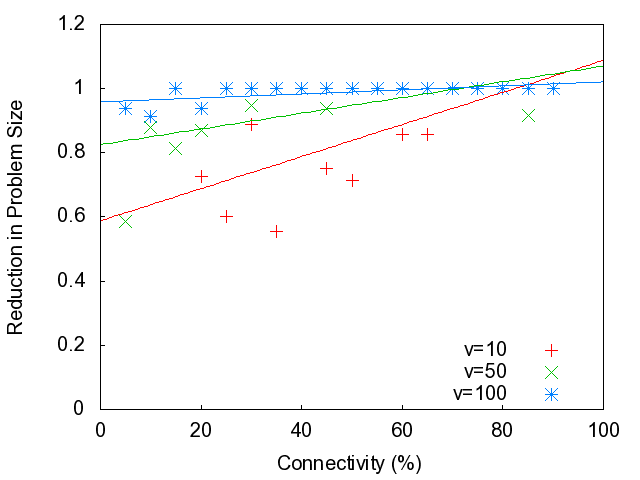
\includegraphics[scale=0.375]{experiments/graph-connectivity.png}
\caption{Comparison of reduction in decomposed problem size for networks with different connectiviy and size}\label{figure:connectivity}
\end{figure}

Figure \ref{figure:connectivity} illustrates the ratio of decomposed problem and original POMDP problem size. For dense graphs of 80\% connectivity decomposition preserves nearly all of the states. However it is possible to eliminate 10\%-15\% percentage of the genes when the network is denser.

This result verifies the expectation that, in sparse networks there are more isolated genes that can be identified and removed from problem description by our method.

\section{Experiments on Comparison of POMDP Formulation with Finite Horizon Models}

For the experimental tests, we build implementations of our POMDP formulation method and two other 
gene regulatory network control problem settings mentioned above. 

For the realization of the optimization method developed by Datta et. al. we used two alternate implementations. 
One of the implementations strictly follows the algorithm proposed by Datta et. al. at \cite{Datta04}. Gene 
regulatory network control problem is formalized as a finite horizon, stochastic optimization problem 
with imprecise knowledge about the system. A dynamic programming algorithm is used to solve the optimization
problem and extracting a policy. We designated this implementation as \textsc{Optimization-1}.

We also implemented the alternative realization of this algorithm, as formulated in \cite{Bryce06} 
by Bryce et.al. This version of the method uses the same algorithm, however suggests an identical  graph search 
instead of dynamic programming. Bryce et.al. used this alternative realization since this realization is more 
similar to their method and it is easier to compare two, then comparing a dynamic programming algorithm with a 
graph search algorithm. We designated this implementation as \textsc{Optimization-2}.

Similarly we also realized the AO* method proposed by Bryce et. al. by implementing 
the graph search algorithm they proposed. Alternative implementation of optimization method and the 
implementation of AO* method share similar components and only differ in the way they expand nodes of 
the search graph. This implementation is designated as \textsc{AO*}.

For our POMDP formulation method we used \emph{Symbolic Perseus} POMDP solver for solving the constructed 
POMDP problem. Symbolic Perseus is a POMDP solver that makes use of a point-based value iteration algorithm
\cite{Poupart05}. It can solve large POMDP problems and the POMDP solving algorithm it uses is an infinite horizon
algorithm. It also uses factored POMDP representation which provides gains in performance and ease of 
defining problems. For working with Symbolic Perseus, our implementation prepares a problem description 
file that is compatible with Symbolic Perseus. Symbolic Perseus can input the problem and produce a policy. 
We designated our approach as \textsc{UHFP} which is an acronym for \fBold{Unbounded} \fBold{Horizon} \fBold{Factored} \fBold{POMDP}.

All four methods are evaluated with a gene regulatory network based on metastatic melanoma data \cite{Bittner00}. 
Kim et.al.  developed a PBN model based on this gene expression data \cite{Kim02}. Datta et.al 
formulated a control problem on a 7-gene version of this PBN formulation. The number of observed genes,
 intervened genes and target genes vary in the different settings of the control problem. This control 
problem is also used by Bryce et.al. for comparison. In this experimental evaluation, we also used this 
problem for comparing the performance of our POMDP formulation with these related work.

For evaluating the alternative algorithms we first solved the control problem and measured processing 
time and memory used in solution process. Then we measured the quality of the solution by running 100 simulations of 
the solution. Total simulation time and average reward are calculated after this simulation.

Since our \textsc{UHFP} method works on an unbounded horizon, we did not solve the control problem for different horizon
values as other methods did. For each problem setting with given number of actions, oberservations and target genes,
we run our solution method only once. Then the generated policy is used in simulations for different horizon
values.

All software components except the POMDP formulation part of our own method work on MATLAB. We used Symbolic 
Perseus for solving our POMDP formulations and Probabilistic Boolean Network Toolbox for formulations 
of other competing methods. POMDP formulation of our method is implemented on Ruby. All experiments are 
carried on Intel Core i7 740QM 1.73 Ghz Processor and 6 GB memory. We used the default memory limitations of MATLAB
as memory limit in our experiments. For each experimental run, we used 30 minutes as time limit.

\subsection{Experimental Results}

\begin{table}
\centering
\scalebox{0.7}{%
\begin{tabular}{|c|c|c|c|c|} \hline
Horizon & Solution Time & Memory Used & Simulation Time & Average Reward \\  \hline
\multicolumn{5}{|c|} {$|A| = 1 , |O| = 1, |T| = 1$} \\  \hline
$h = 3$ & 0.16 s & 395 K & 0.03 s & 8.7 \\  \hline
$h = 6$ & 0.38 s & 570 K & 0.05 s & 19.5 \\  \hline
$h = 9$ & 13.72 s & 17 M & 0.05 s & 46.4 \\  \hline
$h = 12$ & 853.60 s & 1 G & 0.06 s & 64.5 \\  \hline
$h > 12$ & \multicolumn{4}{|c|} {Memory Limit Exceeded}\\  \hline
\multicolumn{5}{|c|} {$|A| = 1 , |O| = 2, |T| = 1$} \\  \hline
$h = 3$ & 0.17 s & 404 K & 0.02 s & 9.8 \\  \hline
$h = 6$ & 6.81 s & 11 M & 0.05 s & 21.6 \\ \hline
$h = 9$ & 3577.26 s & 8 G & 0.53 s & 40.3 \\ \hline
$h > 9$ & \multicolumn{4}{|c|} {Memory Limit Exceeded}\\ \hline
\multicolumn{5}{|c|} {$|A| = 1 , |O| = 3, |T| = 1$} \\ \hline
$h = 3$ & 0.30 s & 475 K & 0.02 s & 13.6 \\ \hline
$h = 6$ & 205.06 s & 704 M & 0.03 s & 33.4 \\ \hline
$h > 6$ & \multicolumn{4}{|c|} {Memory Limit Exceeded}\\ \hline
\multicolumn{5}{|c|} {$|A| = 1 , |O| = 4, |T| = 1$} \\ \hline
$h = 3$ & 0.41 s & 1 M & 0.02 s & 11.4 \\ \hline
$h > 3$ & \multicolumn{4}{|c|} {Memory Limit Exceeded}\\ \hline
\multicolumn{5}{|c|} {$|A| = 1 , |O| = 5, |T| = 1$} \\ \hline
$h = 3$ & 1.25 s & 5 M & 0.02 s & 10.2 \\ \hline
$h > 3$ & \multicolumn{4}{|c|} {Memory Limit Exceeded}\\ \hline
\multicolumn{5}{|c|} {$|A| = 2 , |O| = 1, |T| = 1$} \\ \hline
$h = 3$ & 0.25 s & 535 K  & 0.02 s & 13.9 \\ \hline
$h = 6$ & 1.79 s & 1 M  & 0.05 s & 20.9 \\ \hline
$h = 9$ & 325.41 s & 436 M  & 0.05 s & 42.9 \\ \hline
$h > 9$ & \multicolumn{4}{|c|} {Memory Limit Exceeded}\\ \hline
\multicolumn{5}{|c|} {$|A| = 2 , |O| = 2, |T| = 1$} \\ \hline
$h = 3$ & 0.24 s & 545 K  & 0.02 s & 13 \\ \hline
$h = 6$ & 45.23 s & 84 M  & 0.04 s & -0.4 \\ \hline
$h > 6$ & \multicolumn{4}{|c|} {Memory Limit Exceeded}\\ \hline
\multicolumn{5}{|c|} {$|A| = 2 , |O| = 3, |T| = 1$} \\ \hline
$h = 3$ & 0.35 s & 703 K  & 0.02 s & 14.2 \\ \hline
$h = 6$ & 1630.95 s & 5 G  & 0.07 s & 28 \\ \hline
$h > 6$ & \multicolumn{4}{|c|} {Memory Limit Exceeded}\\ \hline
\multicolumn{5}{|c|} {$|A| = 2 , |O| = 4, |T| = 1$} \\ \hline
$h = 3$ & 0.93 s & 2 M & 0.02 s & 13.1 \\ \hline
$h > 3$ & \multicolumn{4}{|c|} {Memory Limit Exceeded}\\ \hline
\multicolumn{5}{|c|} {$|A| = 2 , |O| = 5, |T| = 1$} \\ \hline
$h = 3$ & 5.71 s & 11 M & 0.03 s & 11.5 \\ \hline
$h > 3$ & \multicolumn{4}{|c|} {Memory Limit Exceeded}\\ \hline
\multicolumn{5}{|c|} {$|A| = 3 , |O| = 1, |T| = 1$} \\ \hline
$h = 3$ & 0.32 s & 655 K & 0.02 s & 9.2 \\ \hline
$h = 6$ & 6.55 s & 6 M & 0.03 s & 24.9 \\ \hline
$h > 6$ & \multicolumn{4}{|c|} {Memory Limit Exceeded}\\ \hline
\multicolumn{5}{|c|} {$|A| = 3 , |O| = 2, |T| = 1$} \\ \hline
$h = 3$ & 0.36 s & 690 K & 0.02 s & 15 \\ \hline
$h = 6$ & 190.53 s & 352 M & 0.03 s & 30.9 \\ \hline
$h > 6$ & \multicolumn{4}{|c|} {Memory Limit Exceeded}\\ \hline
\multicolumn{5}{|c|} {$|A| = 3 , |O| = 3, |T| = 1$} \\ \hline
$h = 3$ & 0.66 s & 971 K & 0.01 s & 15.8 \\ \hline
$h > 3$ & \multicolumn{4}{|c|} {Memory Limit Exceeded}\\ \hline
\multicolumn{5}{|c|} {$|A| = 4 , |O| = 1, |T| = 1$} \\ \hline
$h = 3$ & 0.49 s & 1 M & 0.02 s & 14.5 \\ \hline
$h > 3$ & \multicolumn{4}{|c|} {Memory Limit Exceeded}\\ \hline
\multicolumn{5}{|c|} {$|A| = 4 , |O| = 2, |T| = 1$} \\ \hline
$h = 3$ & 0.93 s & 2 M & 0.03 s & 10.5 \\ \hline
$h > 3$ & \multicolumn{4}{|c|} {Memory Limit Exceeded}\\ \hline
\multicolumn{5}{|c|} {$|A| = 4 , |O| = 3, |T| = 1$} \\ \hline
$h = 3$ & 1.47 s & 3 M & 0.02 s & 12 \\ \hline
$h > 3$ & \multicolumn{4}{|c|} {Memory Limit Exceeded}\\ \hline
\multicolumn{5}{|c|} {$|A| = 5 , |O| = 1, |T| = 1$} \\ \hline
$h = 3$ & 1.51 s & 5 M & 0.02 s & 14.6 \\ \hline
$h > 3$ & \multicolumn{4}{|c|} {Memory Limit Exceeded}\\ \hline
\multicolumn{5}{|c|} {$|A| = 5 , |O| = 2, |T| = 1$} \\ \hline
$h = 3$ & 3.26 s & 11 M & 0.02 s & 13.3\\ \hline
$h > 3$ & \multicolumn{4}{|c|} {Memory Limit Exceeded}\\ \hline
\end{tabular}}
\caption{Experimental Results for OPTIMIZATION-1 Implementation}\label{results:datta1}
\end{table}

\begin{table}
\centering
\scalebox{0.7}{%
\begin{tabular}{|c|c|c|c|c|} \hline
Horizon & Solution Time & Memory Used & Simulation Time & Average Reward \\  \hline
\multicolumn{5}{|c|} {$|A| = 1 , |O| = 1, |T| = 1$} \\  \hline
$h = 3$ & 1.94 s & 943 K & 0.17 s & 14.9 \\  \hline
$h > 3$ & \multicolumn{4}{|c|} {Time Limit Exceeded}\\  \hline
\multicolumn{5}{|c|} {$|A| = 1 , |O| = 2, |T| = 1$} \\  \hline
$h = 3$ & 46.62 s & 5 M & 0.42 s & 12.3 \\  \hline
$h > 3$ & \multicolumn{4}{|c|} {Time Limit Exceeded}\\ \hline
\multicolumn{5}{|c|} {$|A| = 1 , |O| = 3, |T| = 1$} \\ \hline
\multicolumn{5}{|c|} {Time Limit Exceeded}\\ \hline
\multicolumn{5}{|c|} {$|A| = 1 , |O| = 4, |T| = 1$} \\ \hline
\multicolumn{5}{|c|} {Time Limit Exceeded}\\ \hline
\multicolumn{5}{|c|} {$|A| = 1 , |O| = 5, |T| = 1$} \\ \hline
\multicolumn{5}{|c|} {Time Limit Exceeded}\\ \hline
\multicolumn{5}{|c|} {$|A| = 2 , |O| = 1, |T| = 1$} \\  \hline
$h = 3$ & 8.79 s & 2 M & 0.27 s & 13.2 \\  \hline
$h > 3$ & \multicolumn{4}{|c|} {Time Limit Exceeded}\\  \hline
\multicolumn{5}{|c|} {$|A| = 2 , |O| = 2, |T| = 1$} \\  \hline
$h = 3$ & 539.92 s & 15 M & 0.64 s & 5.12 \\  \hline
$h > 3$ & \multicolumn{4}{|c|} {Time Limit Exceeded}\\  \hline
\multicolumn{5}{|c|} {$|A| = 2 , |O| = 3, |T| = 1$} \\ \hline
\multicolumn{5}{|c|} {Time Limit Exceeded}\\ \hline
\multicolumn{5}{|c|} {$|A| = 2 , |O| = 4, |T| = 1$} \\ \hline
\multicolumn{5}{|c|} {Time Limit Exceeded}\\ \hline
\multicolumn{5}{|c|} {$|A| = 2 , |O| = 5, |T| = 1$} \\ \hline
\multicolumn{5}{|c|} {Time Limit Exceeded}\\ \hline
\multicolumn{5}{|c|} {$|A| = 3 , |O| = 1, |T| = 1$} \\  \hline
$h = 3$ & 44.63 s & 5 M & 0.30 s & 12.3 \\  \hline
$h > 3$ & \multicolumn{4}{|c|} {Time Limit Exceeded}\\  \hline
\multicolumn{5}{|c|} {$|A| = 3 , |O| = 2, |T| = 1$} \\ \hline
\multicolumn{5}{|c|} {Time Limit Exceeded}\\ \hline
\multicolumn{5}{|c|} {$|A| = 3 , |O| = 3, |T| = 1$} \\ \hline
\multicolumn{5}{|c|} {Time Limit Exceeded}\\ \hline
\multicolumn{5}{|c|} {$|A| = 4 , |O| = 1, |T| = 1$} \\  \hline
$h = 3$ & 177.07 s & 9 M & 0.39 s & 13.1 \\  \hline
$h > 3$ & \multicolumn{4}{|c|} {Time Limit Exceeded}\\  \hline
\multicolumn{5}{|c|} {$|A| = 4 , |O| = 2, |T| = 1$} \\ \hline
\multicolumn{5}{|c|} {Time Limit Exceeded}\\ \hline
\multicolumn{5}{|c|} {$|A| = 4 , |O| = 3, |T| = 1$} \\ \hline
\multicolumn{5}{|c|} {Time Limit Exceeded}\\ \hline
\multicolumn{5}{|c|} {$|A| = 5 , |O| = 1, |T| = 1$} \\  \hline
$h = 3$ & 533.62 s & 15 M & 0.51 s & 13.2 \\  \hline
$h > 3$ & \multicolumn{4}{|c|} {Time Limit Exceeded}\\  \hline
\multicolumn{5}{|c|} {$|A| = 5 , |O| = 2, |T| = 1$} \\ \hline
\multicolumn{5}{|c|} {Time Limit Exceeded}\\ \hline
\end{tabular}}
\caption{Experimental Results for OPTIMIZATION-2 Implementation}\label{results:datta2}
\end{table}

\begin{table}
\centering
\scalebox{0.7}{%
\begin{tabular}{|c|c|c|c|c|} \hline
Horizon & Solution Time & Memory Used & Simulation Time & Average Reward \\  \hline
\multicolumn{5}{|c|} {$|A| = 1 , |O| = 1, |T| = 1$} \\  \hline
$h = 3$ & 0.44 s & 527 K & 0.10 s & 12.6 \\  \hline
$h = 6$ & 19.14 s & 2 M & 0.38 s & 23.94 \\  \hline
$h > 6$ & \multicolumn{4}{|c|} {Time Limit Exceeded}\\  \hline
\multicolumn{5}{|c|} {$|A| = 1 , |O| = 2, |T| = 1$} \\  \hline
$h = 3$ & 6.86 s & 1 M & 0.12 s & 12.54 \\  \hline
$h > 3$ & \multicolumn{4}{|c|} {Time Limit Exceeded}\\ \hline
\multicolumn{5}{|c|} {$|A| = 1 , |O| = 3, |T| = 1$} \\  \hline
$h = 3$ & 625.35 s & 10 M & 0.14 s & 12.08 \\  \hline
$h > 3$ & \multicolumn{4}{|c|} {Time Limit Exceeded}\\ \hline
\multicolumn{5}{|c|} {$|A| = 1 , |O| = 4, |T| = 1$} \\ \hline
\multicolumn{5}{|c|} {Time Limit Exceeded}\\ \hline
\multicolumn{5}{|c|} {$|A| = 1 , |O| = 5, |T| = 1$} \\ \hline
\multicolumn{5}{|c|} {Time Limit Exceeded}\\ \hline
\multicolumn{5}{|c|} {$|A| = 2 , |O| = 1, |T| = 1$} \\  \hline
$h = 3$ & 0.63 s & 732 K & 0.14 s & 11.4 \\  \hline
$h = 6$ & 25.91 s & 3 M & 0.40 s & 24.12 \\  \hline
$h > 6$ & \multicolumn{4}{|c|} {Time Limit Exceeded}\\  \hline
\multicolumn{5}{|c|} {$|A| = 2 , |O| = 2, |T| = 1$} \\  \hline
$h = 3$ & 10.41 s & 2 M & 0.11 s & 6.52 \\  \hline
$h > 3$ & \multicolumn{4}{|c|} {Time Limit Exceeded}\\  \hline
\multicolumn{5}{|c|} {$|A| = 2 , |O| = 3, |T| = 1$} \\  \hline
$h = 3$ & 980.69 s & 13 M & 0.15 s & 12.3 \\  \hline
$h > 3$ & \multicolumn{4}{|c|} {Time Limit Exceeded}\\  \hline
\multicolumn{5}{|c|} {$|A| = 2 , |O| = 4, |T| = 1$} \\ \hline
\multicolumn{5}{|c|} {Time Limit Exceeded}\\ \hline
\multicolumn{5}{|c|} {$|A| = 2 , |O| = 5, |T| = 1$} \\ \hline
\multicolumn{5}{|c|} {Time Limit Exceeded}\\ \hline
\multicolumn{5}{|c|} {$|A| = 3 , |O| = 1, |T| = 1$} \\  \hline
$h = 3$ & 0.81 s & 936 K & 0.12 s & 12.2 \\  \hline
$h = 6$ & 42.03 s & 4 M & 0.36 s & 32.83 \\  \hline
$h > 6$ & \multicolumn{4}{|c|} {Time Limit Exceeded}\\  \hline
\multicolumn{5}{|c|} {$|A| = 3 , |O| = 2, |T| = 1$} \\  \hline
$h = 3$ & 13.28 s & 2 M & 0.11 s & 14.7 \\  \hline
$h > 3$ & \multicolumn{4}{|c|} {Time Limit Exceeded}\\  \hline
\multicolumn{5}{|c|} {$|A| = 3 , |O| = 3, |T| = 1$} \\  \hline
$h = 3$ & 1121.24 s & 16 M & 0.15 s & 15.82 \\  \hline
$h > 3$ & \multicolumn{4}{|c|} {Time Limit Exceeded}\\  \hline
\multicolumn{5}{|c|} {$|A| = 3 , |O| = 4, |T| = 1$} \\ \hline
\multicolumn{5}{|c|} {Time Limit Exceeded}\\ \hline
\multicolumn{5}{|c|} {$|A| = 4 , |O| = 1, |T| = 1$} \\  \hline
$h = 3$ & 1.02 s & 1 M & 0.12 s & 11.24 \\  \hline
$h = 6$ & 44.10 s & 4 M & 0.37 s & 18.75 \\  \hline
$h > 6$ & \multicolumn{4}{|c|} {Time Limit Exceeded}\\  \hline
\multicolumn{5}{|c|} {$|A| = 4 , |O| = 2, |T| = 1$} \\  \hline
$h = 3$ & 19.82 s & 3 M & 0.12 s & 10.6 \\  \hline
$h > 3$ & \multicolumn{4}{|c|} {Time Limit Exceeded}\\  \hline
\multicolumn{5}{|c|} {$|A| = 4 , |O| = 3, |T| = 1$} \\ \hline
\multicolumn{5}{|c|} {Time Limit Exceeded}\\ \hline
\multicolumn{5}{|c|} {$|A| = 5 , |O| = 1, |T| = 1$} \\  \hline
$h = 3$ & 1.26 s & 1 M & 0.19 s & 11.18 \\  \hline
$h = 6$ & 63.35 s & 5 M & 0.37 s & 36.8 \\  \hline
$h > 6$ & \multicolumn{4}{|c|} {Time Limit Exceeded}\\  \hline
\multicolumn{5}{|c|} {$|A| = 5 , |O| = 2, |T| = 1$} \\ \hline
$h = 3$ & 28.93 s & 4 M & 0.13 s & 12.98 \\  \hline
$h > 3$ & \multicolumn{4}{|c|} {Time Limit Exceeded}\\  \hline
\end{tabular}}
\caption{Experimental Results for AO* Implementation}\label{results:bryce}
\end{table}

\begin{table}
\centering
\scalebox{0.6}{%
\begin{tabular}{|c|c|c|c|c|} \hline
Horizon & Solution Time & Memory Used & Simulation Time & Average Reward \\  \hline
& \multicolumn{4}{|c|} {$|A| = 1 , |O| = 1, |T| = 1$} \\  \hline
$h = 3$ & \multirow{7}{*}{8.34 s} & \multirow{7}{*}{26 K} & 0.95 s & 13.28 \\  
$h = 6$ &  &  & 1.89 s & 21.65 \\  
$h = 9$ &  &  & 2.64 s & 28.12 \\ 
$h = 12$ &  &  & 3.42 s & 33.22 \\ 
$h = 15$ &  &  & 4.30 s & 37.65 \\  
$h = 18$ &  &  & 5.28 s & 40.80 \\ 
$h = 21$ &  &  & 5.86 s & 42.79 \\  \hline
& \multicolumn{4}{|c|} {$|A| = 1 , |O| = 2, |T| = 1$} \\  \hline
$h = 3$ & \multirow{7}{*}{8.68 s} & \multirow{7}{*}{64 K} & 1.16 s & 13.44 \\  
$h = 6$ &  &  & 2.25 s & 23.50 \\  
$h = 9$ &  &  & 2.66 s & 31.34 \\  
$h = 12$ &  &  & 3.31 s & 36.94 \\ 
$h = 15$ &  &  & 3.88 s & 40.83 \\ 
$h = 18$ &  &  & 4.55 s & 43.86 \\ 
$h = 21$ &  &  & 5.21 s & 45.90 \\  \hline
& \multicolumn{4}{|c|} {$|A| = 1 , |O| = 3, |T| = 1$} \\  \hline
$h = 3$ & \multirow{7}{*}{8.79 s} & \multirow{7}{*}{66 K} & 0.93 s & 13.28 \\ 
$h = 6$ &  &  & 1.49 s & 23.40 \\  
$h = 9$ &  &  & 2.41 s & 30.93 \\  
$h = 12$ &  &  & 3.00 s & 37.39 \\ 
$h = 15$ &  &  & 3.58 s & 41.64 \\ 
$h = 18$ &  &  & 4.15 s & 44.47 \\ 
$h = 21$ &  &  & 4.81 s & 46.60 \\  \hline
& \multicolumn{4}{|c|} {$|A| = 1 , |O| = 4, |T| = 1$} \\  \hline
$h = 3$ & \multirow{7}{*}{11.03 s} & \multirow{7}{*}{68 K} & 0.82 s & 13.28 \\ 
$h = 6$ &  &  & 1.27 s & 23.15 \\ 
$h = 9$ &  &  & 1.80 s & 30.10 \\ 
$h = 12$ &  &  & 2.39 s & 35.45 \\
$h = 15$ &  &  & 2.97 s & 39.12 \\
$h = 18$ &  &  & 3.55 s & 40.32 \\
$h = 21$ &  &  & 4.00 s & 41.27 \\
& \multicolumn{4}{|c|} {$|A| = 1 , |O| = 5, |T| = 1$} \\  \hline
$h = 3$ & \multirow{7}{*}{16.80 s} & \multirow{7}{*}{70 K} & 0.86 s & 13.28 \\ 
$h = 6$ &  &  & 1.46 s & 22.93 \\ 
$h = 9$ &  &  & 2.08 s & 30.28 \\ 
$h = 12$ &  &  & 2.55 s & 35.88 \\ 
$h = 15$ &  &  & 2.99 s & 39.40 \\ 
$h = 18$ &  &  & 3.47 s & 41.85 \\ 
$h = 21$ &  &  & 3.95 s & 43.73 \\  \hline
& \multicolumn{4}{|c|} {$|A| = 2 , |O| = 1, |T| = 1$} \\  \hline
$h = 3$ & \multirow{7}{*}{9.32 s} & \multirow{7}{*}{27 K} & 0.95 s & 13.28 \\  
$h = 6$ &  &  & 1.96 s & 21.65 \\ 
$h = 9$ &  &  & 2.76 s & 28.12 \\ 
$h = 12$ &  &  & 3.63 s & 33.22 \\
$h = 15$ &  &  & 4.48 s & 47.65 \\ 
$h = 18$ &  &  & 5.38 s & 40.80 \\ 
$h = 21$ &  &  & 6.22 s & 42.79 \\  \hline
& \multicolumn{4}{|c|} {$|A| = 2 , |O| = 2, |T| = 1$} \\  \hline
$h = 3$ & \multirow{7}{*}{8.42 s} & \multirow{7}{*}{67 K} & 1.34 s & 13.44 \\ 
$h = 6$ &  &  & 2.02 s & 23.50 \\ 
$h = 9$ &  &  & 2.77 s & 31.34 \\ 
$h = 12$ &  &  & 3.46 s & 36.94 \\ 
$h = 15$ &  &  & 4.19 s & 40.83 \\ 
$h = 18$ &  &  & 4.96 s & 43.86 \\ 
$h = 21$ &  &  & 5.73 s & 45.90 \\  \hline
& \multicolumn{4}{|c|} {$|A| = 2 , |O| = 3, |T| = 1$} \\  \hline
$h = 3$ & \multirow{7}{*}{10.35 s} & \multirow{7}{*}{68 K} & 1.05 s & 13.28 \\  
$h = 6$ &  &  & 1.67 s & 23.40 \\  
$h = 9$ &  &  & 2.38 s & 30.94 \\ 
$h = 12$ &  &  & 2.88 s & 37.39 \\
$h = 15$ &  &  & 4.33 s & 41.64 \\
$h = 18$ &  &  & 4.06 s & 44.47 \\
$h = 21$ &  &  & 4.68 s & 46.60 \\  \hline
& \multicolumn{4}{|c|} {$|A| = 2 , |O| = 4, |T| = 1$} \\  \hline
$h = 3$ & \multirow{7}{*}{23.74 s} & \multirow{7}{*}{61 K} & 0.92 s & 13.28 \\ 
$h = 6$ &  &  & 1.64 s & 23.15 \\
$h = 9$ &  &  & 2.34 s & 30.10 \\
$h = 12$ &  &  & 3.78 s & 35.45 \\ 
$h = 15$ &  &  & 3.36 s & 39.12 \\ 
$h = 18$ &  &  & 3.92 s & 40.32 \\
$h = 21$ &  &  & 4.49 s & 41.27 \\ \hline
& \multicolumn{4}{|c|} {$|A| = 2 , |O| = 5, |T| = 1$} \\  \hline
$h = 3$ & \multirow{7}{*}{20.03 s} & \multirow{7}{*}{71 K} & 0.90 s & 13.28 \\ 
$h = 6$ &  &  & 1.49 s & 22.93 \\ 
$h = 9$ &  &  & 2.21 s & 30.28 \\ 
$h = 12$ &  &  & 2.81 s & 35.88 \\
$h = 15$ &  &  & 3.17 s & 39.40 \\
$h = 18$ &  &  & 3.98 s & 41.85 \\
$h = 21$ &  &  & 4.32 s & 43.73 \\ \hline
\end{tabular}}
\caption{Experimental Results for \textsc{UHFP} Implementation Part 1}\label{results:uhfp1}
\end{table}

\begin{table}
\centering
\scalebox{0.6}{%
\begin{tabular}{|c|c|c|c|c|} \hline
Horizon & Solution Time & Memory Used & Simulation Time & Average Reward \\  \hline
& \multicolumn{4}{|c|} {$|A| = 3 , |O| = 1, |T| = 1$} \\  \hline
$h = 3$ & \multirow{7}{*}{10.32 s} & \multirow{7}{*}{30 K} & 0.95 s & 13.28 \\ 
$h = 6$ &  &  & 2.10 s & 21.65 \\ 
$h = 9$ &  &  & 2.86 s & 28.12 \\ 
$h = 12$ &  &  & 3.62 s & 33.22 \\
$h = 15$ &  &  & 4.57 s & 37.65 \\
$h = 18$ &  &  & 5.40 s & 40.80 \\
$h = 21$ &  &  & 6.12 s & 42.79 \\ \hline
& \multicolumn{4}{|c|} {$|A| = 3 , |O| = 2, |T| = 1$} \\  \hline
$h = 3$ & \multirow{7}{*}{10.06 s} & \multirow{7}{*}{68 K} & 1.11 s & 13.44 \\
$h = 6$ &  &  & 2.98 s & 23.50 \\
$h = 9$ &  &  & 2.67 s & 31.34 \\
$h = 12$ &  &  & 3.28 s & 36.94 \\
$h = 15$ &  &  & 4.06 s & 40.83 \\
$h = 18$ &  &  & 4.62 s & 43.86 \\
$h = 21$ &  &  & 5.26 s & 45.90 \\ \hline
& \multicolumn{4}{|c|} {$|A| = 3 , |O| = 3, |T| = 1$} \\  \hline
$h = 3$ & \multirow{7}{*}{13.51 s} & \multirow{7}{*}{70 K} & 1.08 s & 13.28 \\ 
$h = 6$ &  &  & 1.91 s & 23.40 \\
$h = 9$ &  &  & 2.60 s & 30.94 \\
$h = 12$ &  &  & 3.23 s & 37.39 \\
$h = 15$ &  &  & 4.10 s & 41.63 \\
$h = 18$ &  &  & 4.47 s & 44.47 \\
$h = 21$ &  &  & 5.16 s & 46.60 \\ \hline
& \multicolumn{4}{|c|} {$|A| = 3 , |O| = 4, |T| = 1$} \\  \hline
$h = 3$ & \multirow{7}{*}{15.35 s} & \multirow{7}{*}{72 K} & 1.01 s & 13.28 \\
$h = 6$ &  &  & 1.72 s & 23.15 \\
$h = 9$ &  &  & 2.46 s & 30.10 \\
$h = 12$ &  &  & 3.11 s & 35.45 \\
$h = 15$ &  &  & 3.60 s & 39.12 \\
$h = 18$ &  &  & 4.30 s & 40.31 \\
$h = 21$ &  &  & 4.83 s & 41.27 \\ \hline
& \multicolumn{4}{|c|} {$|A| = 4 , |O| = 1, |T| = 1$} \\  \hline
$h = 3$ & \multirow{7}{*}{11.61 s} & \multirow{7}{*}{31 K} & 1.09 s & 13.28 \\
$h = 6$ &  &  & 2.10 s & 21.65 \\
$h = 9$ &  &  & 2.84 s & 28.12 \\
$h = 12$ &  &  & 3.79 s & 33.22 \\
$h = 15$ &  &  & 4.61 s & 37.65 \\
$h = 18$ &  &  & 5.40 s & 40.80 \\
$h = 21$ &  &  & 6.20 s & 42.79 \\ \hline
& \multicolumn{4}{|c|} {$|A| = 4 , |O| = 2, |T| = 1$} \\  \hline
$h = 3$ & \multirow{7}{*}{12.12 s} & \multirow{7}{*}{70 K} & 1.32 s & 13.44 \\
$h = 6$ &  &  & 2.49 s & 23.50 \\
$h = 9$ &  &  & 3.66 s & 31.34 \\
$h = 12$ &  &  & 4.24 s & 36.94 \\
$h = 15$ &  &  & 4.99 s & 40.83 \\
$h = 18$ &  &  & 6.06 s & 43.86 \\
$h = 21$ &  &  & 6.90 s & 45.90 \\ \hline
& \multicolumn{4}{|c|} {$|A| = 4 , |O| = 3, |T| = 1$} \\  \hline
$h = 3$ & \multirow{7}{*}{12.67 s} & \multirow{7}{*}{71 K} & 1.12 s & 13.28 \\
$h = 6$ &  &  & 2.13 s & 23.40 \\
$h = 9$ &  &  & 2.95 s & 30.94 \\
$h = 12$ &  &  & 3.81 s & 37.39 \\
$h = 15$ &  &  & 4.58 s & 41.64 \\
$h = 18$ &  &  & 5.36 s & 44.47 \\
$h = 21$ &  &  & 6.23 s & 46.60 \\ \hline
& \multicolumn{4}{|c|} {$|A| = 5 , |O| = 1, |T| = 1$} \\  \hline
$h = 3$ & \multirow{7}{*}{12.50 s} & \multirow{7}{*}{33 K} & 1.10 s & 13.28 \\
$h = 6$ &  &  & 2.05 s & 21.64 \\
$h = 9$ &  &  & 2.86 s & 28.12 \\
$h = 12$ &  &  & 3.63 s & 33.22 \\
$h = 15$ &  &  & 4.52 s & 37.65 \\
$h = 18$ &  &  & 5.42 s & 40.80 \\
$h = 21$ &  &  & 6.25 s & 42.79 \\ \hline
& \multicolumn{4}{|c|} {$|A| = 5 , |O| = 2, |T| = 1$} \\  \hline
$h = 3$ & \multirow{7}{*}{11.99 s} & \multirow{7}{*}{72 K} & 1.23 s & 13.44 \\
$h = 6$ &  &  & 2.16 s & 23.50 \\
$h = 9$ &  &  & 2.95 s & 31.34 \\
$h = 12$ &  &  & 3.64 s & 36.94 \\
$h = 15$ &  &  & 4.39 s & 40.83 \\
$h = 18$ &  &  & 5.14 s & 43.86 \\
$h = 21$ &  &  & 5.90 s & 45.90 \\ \hline
\end{tabular}}
\caption{Experimental Results for \textsc{UHFP} Implementation Part 2}\label{results:uhfp2}
\end{table}

Tables \ref{results:datta1}-\ref{results:uhfp2} present the results of the experiments we run on four 
approaches. Each table present four metric for the performance of an algorithm. These metrics are solution  
time for the problem, memory used while solving the problem, simulation time and average reward received 
at simulation.

In all experiments, solution time is the time to build the problem description and generate the policy. As the number of actions and observations increase, the problem gets more complicated and solution time typically increases for all methods in our experiment. This increase is very fast for both optimization implementations and \textsc{AO*} algorithm. None of these algorithms produce policies in given time with $h> 12$, even in the simple setting of single action and single observation. However, \textsc{UHFP} method calculates the policy without considering the horizon value, thus the solution time does not exceed 30 seconds even in the most complex problem setting and high horizon values ($h = 21$)

Memory column in experimental results also give hints on the scalability of the approaches. \textsc{optimization-1} implementation scales better than \textsc{optimization-2} implementation, because it extensively uses dynamic programming tables that might get as big as 8 GBs. When the same algorithm is implemented with less storage usage the scalability drops significantly. \textsc{AO*} algorithm is similar to the \textsc{optimization-2} implementation in memory use. However, the most important aspect of this algorithm is the pruning parts of the state space, which can be observed in memory usage values. \textsc{\textsc{UHFP}} method uses significantly less memory then all other methods considered. 

Simulation phase calculates the average reward gained by the  policy constructed. The time for this phase is similar for all approaches. Note that for high horizon values, where \textsc{UHFP} can successfully generate policies, this phase takes more time. This is natural since the length of the simulation is directly proportional to the length of horizon. \textsc{UHFP} implementation uses the POMDP planner for the simulation phase too and this also brings a little overhead to the length of simulation.

Similarly the average reward gained at simulation is similar for all approaches. Note that the average is taken on the number of runs and thus as the horizon increases it is expected that average reward increases too. 

Most significant outcome of the experiments is the comparison of the scalability of methods. 
Optimization methods and AO* algorithm scale poorly as the horizon increases. Especially the optimization 
methods fail to produce any results as $A \cup O$ gets bigger.

Our method, named as \textsc{UHFP} (Unbounded Horizon Factored POMDP), is not effected from the horizon value and 
when horizon is increased it clearly outperforms the alternate approaches.

However our \textsc{UHFP} approach does not sacrifice from the solution quality as average rewards clearly depicts. The average reward received does not decrease even for high horizon values.

